\documentclass[a4paper,12pt]{article}
\usepackage[utf8]{inputenc}
\usepackage{graphicx}
\usepackage{hyperref}
\usepackage{amsmath}
\usepackage{geometry}
\usepackage{float}
\usepackage{titlesec}
\usepackage{enumitem}
\usepackage{caption}
\geometry{margin=2.5cm}

\titleformat{\section}{\large\bfseries}{\thesection}{1em}{}
\titleformat{\subsection}{\normalsize\bfseries}{\thesubsection}{1em}{}

\title{\textbf{Documentazione UniSocial}\\\large Corso di Fondamenti del Web – A.A. 2023/2024}
\author{Studenti: Lorenzo Verdura, Luca Cocito}
\date{}

\begin{document}

\maketitle

\section{Scenario applicativo}
L’applicazione sviluppata rappresenta una \textbf{piattaforma sociale web} che consente agli utenti di creare un profilo, pubblicare contenuti testuali, interagire con i post tramite \textit{like}, salvataggi e commenti, oltre che ricevere notifiche in tempo reale.  
L’obiettivo è simulare le principali funzionalità di un piccolo social network, con particolare attenzione alla gestione sicura dell’autenticazione, alla comunicazione client–server e all’aggiornamento in tempo reale dei dati.

Lo scenario applicativo prevede due principali attori:
\begin{itemize}
    \item \textbf{Utente non autenticato:} può registrarsi o effettuare il login.
    \item \textbf{Utente autenticato:} può creare post, visualizzare i propri e quelli degli altri utenti, interagire con essi e ricevere notifiche in tempo reale.
\end{itemize}

\section{Architettura dell’applicazione}
L’applicazione è strutturata secondo l’architettura classica di una \textbf{Single Page Application (SPA)} basata su React per il frontend e Node.js/Express per il backend, con un database MongoDB per la persistenza dei dati.  
È inoltre previsto l’uso di \textbf{Socket.IO} per la gestione degli eventi in tempo reale, come le notifiche di like o commento.

\subsection{Componenti principali}
\begin{itemize}
    \item \textbf{Frontend:} realizzato in React, si occupa della gestione delle interfacce, della navigazione client-side e delle chiamate alle API REST mediante Axios.
    \item \textbf{Backend:} realizzato in Node.js con Express, fornisce le API RESTful per l’autenticazione, la gestione dei post e delle interazioni. Utilizza \textit{jsonwebtoken} per la generazione dei token e \textit{cookie HttpOnly} per la sicurezza delle sessioni.
    \item \textbf{Database:} MongoDB, ospitato in cloud (MongoDB Atlas), utilizzato per memorizzare utenti, post, commenti e notifiche.
    \item \textbf{Socket Server:} integrato nel backend per gestire in tempo reale eventi come notifiche o aggiornamenti dinamici.
\end{itemize}

\section{Diagramma UML dei casi d’uso}
\begin{figure}[H]
    \centering
    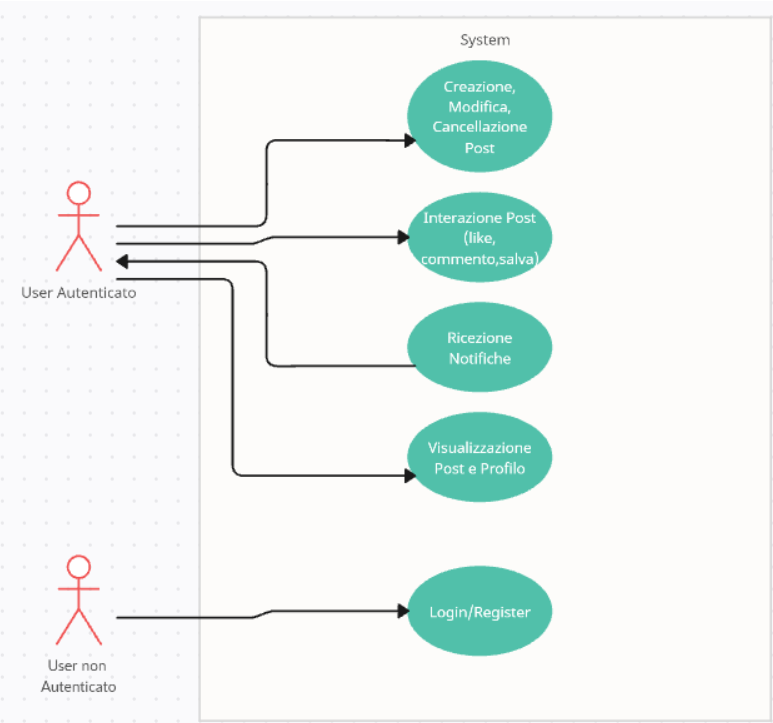
\includegraphics[width=0.8\textwidth]{usecase.png}
    \caption{Diagramma UML dei casi d’uso principali dell’applicazione}
    \label{fig:usecase}
\end{figure}

\noindent
Nel diagramma sono evidenziati i seguenti casi d’uso principali:
\begin{itemize}
    \item Registrazione e login utente
    \item Creazione, modifica e cancellazione di un post
    \item Interazione con i post (like, salvataggio, commento)
    \item Visualizzazione profilo e post personali
    \item Ricezione notifiche in tempo reale
\end{itemize}

\section{Modello dei dati}
Il modello dei dati è stato progettato per garantire coerenza, scalabilità e semplicità di estensione.

\subsection{Entità principali}
\begin{itemize}
    \item \textbf{User}
    \begin{itemize}
        \item \texttt{\_id}: identificativo univoco
        \item \texttt{username}, \texttt{email}, \texttt{password (hash)}
        \item \texttt{isVerified}, \texttt{verificationToken}
        \item \texttt{createdAt}, \texttt{updatedAt}
    \end{itemize}

    \item \textbf{Post}
    \begin{itemize}
        \item \texttt{\_id}, \texttt{authorId}, \texttt{content}
        \item \texttt{likes}: lista di utenti che hanno messo like
        \item \texttt{savedBy}: lista di utenti che hanno salvato il post
        \item \texttt{createdAt}
    \end{itemize}

    \item \textbf{Comment}
    \begin{itemize}
        \item \texttt{\_id}, \texttt{postId}, \texttt{authorId}, \texttt{text}, \texttt{createdAt}
    \end{itemize}

    \item \textbf{Notification}
    \begin{itemize}
        \item \texttt{\_id}, \texttt{recipientId}, \texttt{senderId}, \texttt{type} (like, comment, follow), \texttt{read}, \texttt{createdAt}
    \end{itemize}
\end{itemize}

\section{Documentazione delle API (Backend)}
Le principali API REST sono organizzate come segue:

\subsection{Autenticazione (/api/auth)}
\begin{itemize}
    \item \texttt{POST /register} – Crea un nuovo utente (richiede username, email e password)
    \item \texttt{POST /login} – Autentica un utente e genera un token JWT
    \item \texttt{GET /logout} – Termina la sessione rimuovendo il cookie di autenticazione
    \item \texttt{GET /verify-email} – Verifica l’indirizzo email dell’utente tramite token univoco
\end{itemize}

\subsection{Utenti (/api/users)}
\begin{itemize}
    \item \texttt{GET /profile} – Restituisce le informazioni dell’utente autenticato
    \item \texttt{GET /:id} – Restituisce i dati pubblici di un utente specifico
\end{itemize}

\subsection{Post (/api/posts)}
\begin{itemize}
    \item \texttt{GET /} – Restituisce tutti i post visibili all’utente
    \item \texttt{POST /create} – Crea un nuovo post
    \item \texttt{PUT /:id/like} – Mette o rimuove un like
    \item \texttt{PUT /:id/save} – Salva o rimuove il post dai preferiti
    \item \texttt{DELETE /:id} – Elimina un post
\end{itemize}

\subsection{Commenti (/api/comments)}
\begin{itemize}
    \item \texttt{POST /:postId} – Aggiunge un commento a un post
    \item \texttt{GET /:postId} – Restituisce i commenti associati a un post
\end{itemize}

\subsection{Notifiche (/api/notifications)}
\begin{itemize}
    \item \texttt{GET /} – Restituisce tutte le notifiche dell’utente
    \item \texttt{PUT /:id/read} – Segna una notifica come letta
\end{itemize}

Tutte le rotte autenticate sono protette da middleware di verifica del token JWT e da cookie HttpOnly per garantire un elevato livello di sicurezza.

\section{Componenti React (Frontend)}
Il frontend è strutturato in componenti modulari, ciascuno con un ruolo ben definito.

\subsection{Componenti principali}
\begin{itemize}
    \item \textbf{App.jsx}: entry point dell’applicazione e gestione del routing.
    \item \textbf{AuthContext.jsx}: fornisce il contesto di autenticazione a tutti i componenti.
    \item \textbf{SocketContext.jsx}: gestisce la connessione Socket.IO per la ricezione di notifiche in tempo reale.
    \item \textbf{HomePage.jsx}: mostra il feed dei post e consente di interagire con essi.
    \item \textbf{ProfilePage.jsx}: visualizza i post creati dall’utente loggato.
    \item \textbf{NotificationPage.jsx}: mostra le notifiche ricevute, aggiornate in tempo reale.
    \item \textbf{PostModal.jsx}: gestisce la creazione di nuovi post.
    \item \textbf{NavBar.jsx} e \textbf{SideBar.jsx}: componenti grafici per la navigazione.
    \item \textbf{VerifyEmail.jsx}: gestisce la conferma dell’indirizzo email tramite token di verifica.
\end{itemize}

Ogni componente comunica con il backend tramite Axios e sfrutta gli \textit{hook} di React per la gestione dello stato e degli effetti collaterali.

\section{Sicurezza e autenticazione}
L’applicazione adotta diverse strategie per garantire un accesso sicuro e la protezione dei dati:
\begin{itemize}
    \item \textbf{Hashing delle password:} con \texttt{bcrypt}.
    \item \textbf{Token JWT e cookie HttpOnly:} per mantenere la sessione.
    \item \textbf{CSRF Protection:} implementata tramite \texttt{csrf-csrf}.
    \item \textbf{Rate Limiting:} per limitare le richieste ripetute.
    \item \textbf{Sanificazione input e headers di sicurezza:} tramite \texttt{helmet}, \texttt{xss-clean} e \texttt{express-mongo-sanitize}.
    \item \textbf{Verifica email:} con token monouso inviato via email.
\end{itemize}

\section{Architettura distribuita e tecniche avanzate}
Il deploy dell’applicazione è basato su tre servizi:
\begin{itemize}
    \item \textbf{Frontend:} su \textit{Vercel}.
    \item \textbf{Backend:} su \textit{Render}.
    \item \textbf{Database:} su \textit{MongoDB Atlas}.
\end{itemize}
La comunicazione tra frontend e backend avviene tramite HTTPS e CORS configurato per accettare solo il dominio ufficiale.  
L’app è containerizzata tramite Docker per semplificare l’avvio in locale.

\section{Interazione real-time con Socket.IO}
Ogni utente autenticato si collega a una stanza identificata dal proprio \texttt{userId}.  
Eventi come like o commenti generano notifiche in tempo reale, inviate con \texttt{socket.emit()} e gestite dal componente \textbf{SocketContext.jsx}.



\section{Tecniche di sviluppo e testing}
\begin{itemize}
    \item Test API tramite Postman.
    \item Test real-time tramite sessioni multiple.
    \item Logging e debugging lato server.
    \item Gestione versionamento con GitHub.
\end{itemize}

\end{document}
